\documentclass[a4paper,11pt]{article}

\usepackage[utf8]{inputenc}

\usepackage{graphicx}
\usepackage{caption}
\usepackage{subcaption}

\usepackage{pgfplots}
\usepackage{float}
\usepackage{hyperref}
\usepackage{soul}
\hypersetup{
    colorlinks=true, % Enable colored links
    linkcolor=black, % Color for internal links
    urlcolor=black,  % Color for external links
    citecolor=black, % Color for citation links
    pdfborder={0 0 0}, % Remove border around links
}
\newcommand{\underlinehref}[2]{%
    \href{#1}{\ul{#2}}%
}
\pgfplotsset{compat=1.18}


\usepackage{minted}

\begin{document}

    \title{
        \textbf{Breadth-first search in C}
    }
    \author{Péter Herczku}
    \date{Fall 2024}

    \maketitle

    \section*{Introduction}

    The task is to implement the breadth-first search algorithm. 
    I completed the assignment using the C programming language.

    \section*{The idea}

    When we need to traverse a tree that is sorted such that smaller elements are to the left and the larger ones are to the right, the depth first algorithm works just fine.
    
    However, what happens if the tree is sorted differently?
    Let's say that our tree has the root value 1, to the left it has two and to the right it is linked to three. Two is linked to four and five, and three is linked to six and seven.
    In this case we cannot use our beloved depth first algorithm, that's why we came up with the idea of breadth-first searching.

    In the breadth-first algorithm, we traverse the tree one layer at a time.
    In our example case it means that we first go through the first level which is the root (1), then we proceed to the second layer and read nodes two and three.
    FInally, we go one level deeper and read the remaining values: 4, 5, 6, and 7.

    This algorithm is simple to imagine but a bit trickier to implement.
    We can use a queue for the purpose: we begin with an empty queue and we enqueue the root element.
    Then on each iteration we dequeue an element from the queue, we print it, then enqueue the children of this element.
    We do this until the queue gets empty.

    We can first try it using pen and paper to see how the algorithm actually works before jumping into the implementation.

    \begin{figure}[H]
        \centering
        \begin{subfigure}[b]{.5\textwidth}
            \centering
            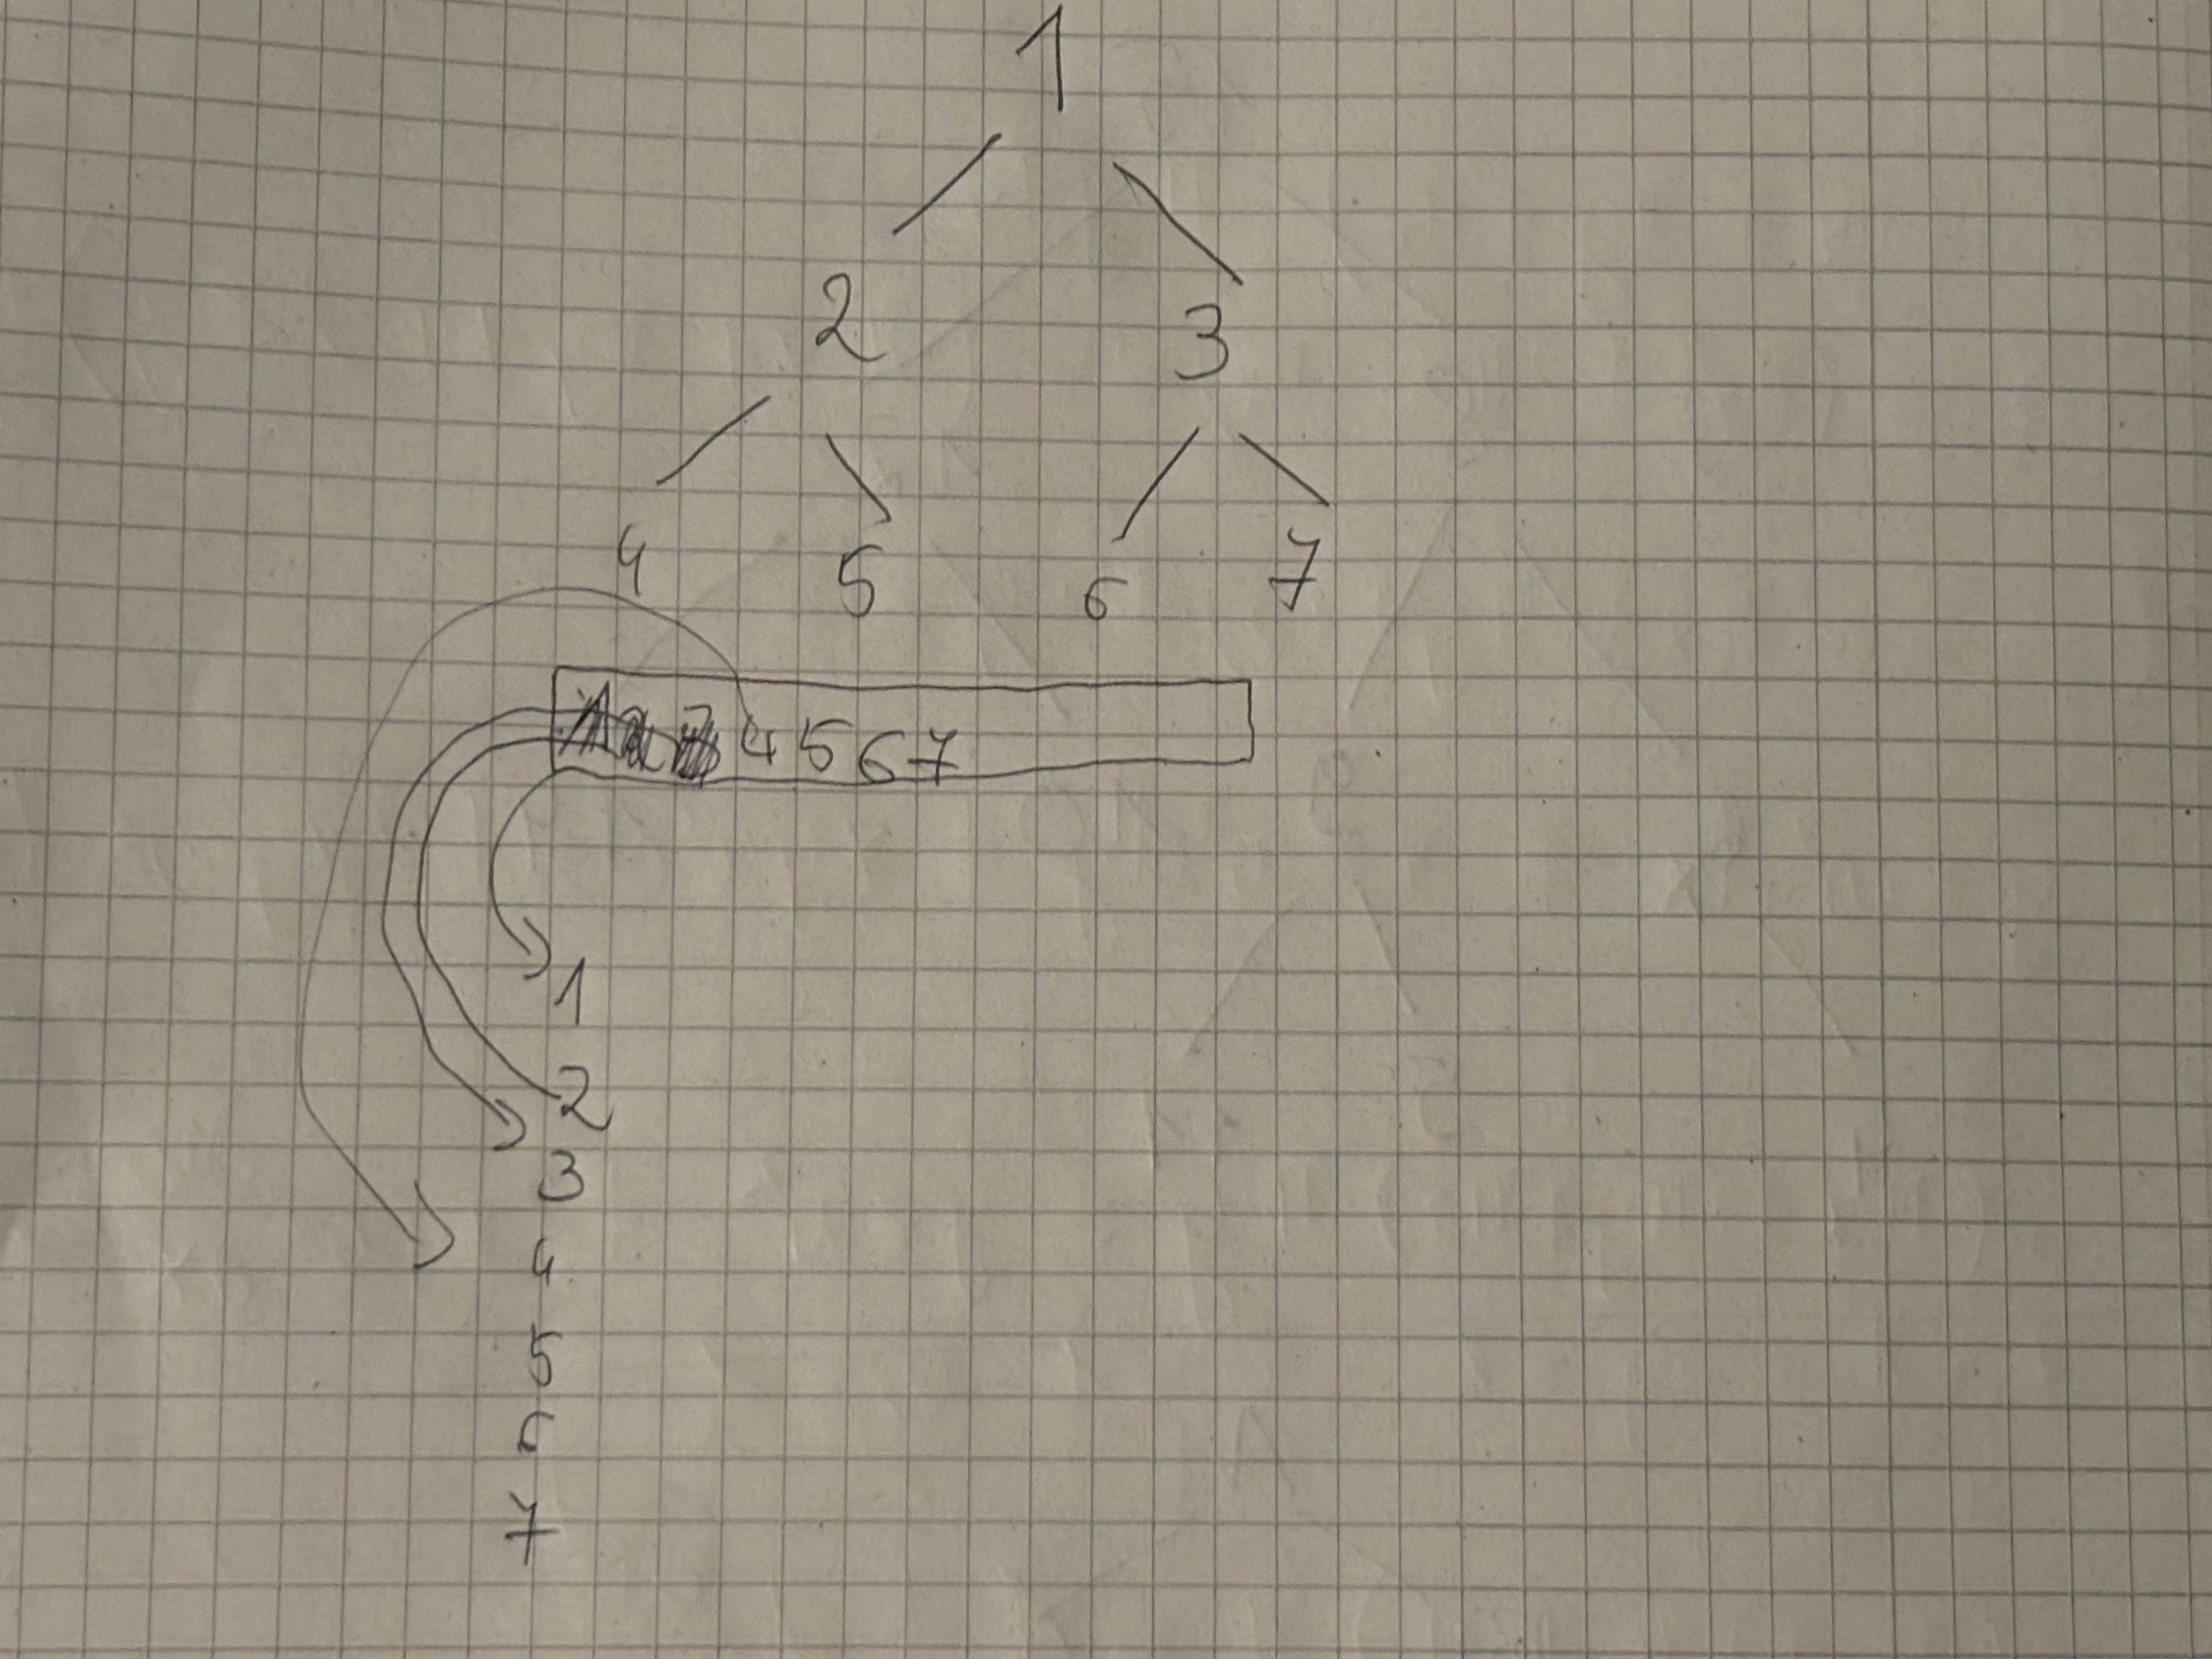
\includegraphics[width=\textwidth]{./picture.jpg} % Adjust width or height as needed
        \end{subfigure}
        \caption{Picture of experimenting on paper}
        \label{fig:graph_1}
    \end{figure}

    Now that we are familiar with the algorithm we can move on to the actual implementation.

    \section*{The queue}

    In the last assignment our queue was holding int values.
    However, in this case our queue needs to hold node structures, where each node represents an element of the tree.
    After modfying the code, we obtained the following structure for the queue:

    \begin{minted}{c}
typedef struct queue_node {
    tree_node* value;
    struct queue_node *next;
} queue_node;

typedef struct queue {
    queue_node *first;
} queue;        
    \end{minted}

    I chose the linked list implementation of the queue, because it's a bit easier to manage.
    Now that we have all the building blocks, we can finally start implementing the breadth first search algorithm.

    \section*{Implementation}

    We have already discussed how the algorithm works in theory, so let's review implementation:
    \begin{minted}{c}
void bfs(tree* tr) {
    queue* q = create_queue();
    enqueue(q, tr->root);
    while (!empty(q)) {
        tree_node* curr = dequeue(q);
        if(curr == NULL) break;
        printf("%d ", curr->value);
        if(curr->left != NULL) enqueue(q, curr->left);
        if(curr->right != NULL) enqueue(q, curr->right);
    }
}  
    \end{minted}

    It's crucial to enqueue the left element first (if possible) and then the right element.
    Otherwise, we would get a false order.

    \section*{Sequence}

    The problem with the current implementation is that it traverses the whole tree even when we are only interested in a portion of it.
    We could create another structure called {\tt sequence}, that would have a method {\tt next}, which would return the next elements one at a time.
    
    This is how our sequence structure looks like:

    \begin{minted}{c}
typedef struct sequence {
    queue* q;
} sequence;
    \end{minted}

    This holds a similar queue to the one used in the breadth-first search method, therefore the implementation of this is quite similar:

    \begin{minted}{c}
int next(sequence* seq) {
    if(empty(seq->q)) return -1;
    tree_node* current = dequeue(seq->q);

    if(current->left != NULL) enqueue(seq->q, current->left);
    if(current->right != NULL) enqueue(seq->q, current->right);
    return current->value;
}
    \end{minted}

    We dequeue an element from the queue, store it in a temporary variable, enqueue its children, then return the value of the temporary variable.
    When the queue is empty, it means that we have gone through every element, and therefore we return an usual value (-1).

    We also need a method that creates a sequence, which could look like this:

    \begin{minted}{c}
sequence* create_sequence(tree *tr) {
    sequence* s = (sequence*)malloc(sizeof(sequence));
    s->q = create_queue();
    if(tr->root != NULL) enqueue(s->q, tr->root);
    return s;
}
    \end{minted}

    If we add a new element to the tree, but its parent has already been dequeued, then the sequence will not provide us the newly added node.
    This is because when we dequeued the parent element it means that we had enqueued the children as well, but the new node had not been added.
    
    Similarly, if we remove a node that has been already enqueued, the sequence will still provide us the removed node, but as long as we are removing the node before enqueuing it, we're fine.

    \section*{GitHub}
    I have uploaded the full project to \underlinehref{https://github.com/peterherczku/ID1021/tree/main/assignment-7-C}{my github repository}, where we can find the code used to make this report.

\end{document}
